\documentclass[12pt,a4paper]{ctexart}
\usepackage[margin=1in]{geometry}
\usepackage{setspace}
\usepackage{booktabs}
\usepackage{longtable}
\usepackage{array}
\usepackage{amsmath,amssymb}
\usepackage{hyperref}
\usepackage{enumitem}
\usepackage{graphicx}
\usepackage{float}
\usepackage{subcaption}

\IfFontExistsTF{Times New Roman}
  {\setmainfont{Times New Roman}}
  {\setmainfont{TeX Gyre Termes}}

% 中文：標楷體 BiauKai
\IfFontExistsTF{BiauKai}
  {\setCJKmainfont[AutoFakeBold=2,AutoFakeSlant=.2]{BiauKai}}
  {\IfFontExistsTF{DFKai-SB}
    {\setCJKmainfont[AutoFakeBold=2,AutoFakeSlant=.2]{DFKai-SB}}
    {\setCJKmainfont[AutoFakeBold=2,AutoFakeSlant=.2]{標楷體}}}
\IfFontExistsTF{BiauKai}
  {\setCJKsansfont[AutoFakeBold=2,AutoFakeSlant=.2]{BiauKai}}
  {\setCJKsansfont[AutoFakeBold=2,AutoFakeSlant=.2]{DFKai-SB}}
\IfFontExistsTF{BiauKai}
  {\setCJKmonofont{BiauKai}}
  {\setCJKmonofont{DFKai-SB}}

\renewcommand{\contentsname}{目錄}
\renewcommand{\refname}{參考文獻}
\renewcommand{\figurename}{圖}
\renewcommand{\tablename}{表}
\renewcommand{\appendixname}{附錄}

\setstretch{1.3}
\setlength{\parskip}{0.5em}
\setlength{\parindent}{2em}
\newcolumntype{L}[1]{>{\raggedright\arraybackslash}p{#1}}

\title{Booking.com 社群文字特徵與互動成效完整結果報告\\[0.3em]
\large 第 5.0.0 版（新增 Negative Binomial 穩健性檢驗）\\[0.3em]
\small 產出時間：2026 年 5 月 7 日}
\author{}
\date{\today}

\begin{document}
\maketitle
\tableofcontents
\newpage

\section*{執行摘要}
\addcontentsline{toc}{section}{執行摘要}

本報告呈現 Booking.com 社群媒體互動研究第 5.0.0 版之完整統計結果。本版主要規格與第 4.0.0 版完全一致，仍採用以 $\ln(1+\text{Engagement})$ 為依變數、HC1 異質變異數穩健標準誤之 OLS 對數線性迴歸。第 5.0.0 版的方法學增量在於新增一項\textbf{負二項（Negative Binomial, NB2）穩健性檢驗}：以同樣的八個解釋變數，在原始整數互動次數上重新估計同一模型，透過對 Poisson 的概似比檢定評估過度離散，並比較兩種函數型式下五項焦點假說的決策一致性。

OLS 結果與第 4.0.0 版完全一致（$N=766$，係數、$R^2=0.5119$、$F(8,757)=76.68$ 全部複現）。NB 穩健性檢驗確認資料具極度過度離散（$\hat\alpha=20.21$，對 Poisson 之 LR 統計量 $=71{,}095$，$p<.0001$），\textbf{五項焦點假說中有四項在 OLS 與 NB 之間決策一致（H1、H2、H4、H5）}。唯一出現分歧的是 H3（情感效價）：OLS 下顯著（$p=.016$），NB 下接近邊際（$p=.100$），符號相同但精度有所削減。圖片、@提及與標籤的效果在兩個模型中皆穩定且強。我們將分歧透明地呈現，而非事後挑選有利模型。

NB 模型採用「固定 $\hat\alpha$」之 GLM 規格，$\hat\alpha$ 由邊際分布的動差估計式 $\hat\alpha_{\text{MoM}}=(s^2(Y)-\bar Y)/\bar Y^2$ 決定。Cameron--Trivedi（1990）輔助迴歸式 $\hat\alpha_{\text{CT}}$ 亦一併報告，僅供診斷用途。本資料集邊際變異數約為平均數之 $850$ 倍，使聯合 NB MLE 對 $\alpha$ 的識別度極低，動差式 GLM 是教科書中於此情境最穩定的選擇。

\section{研究架構}

\subsection{研究問題}
\textbf{Booking.com 在 X 上的貼文，其文字特徵如何影響社群互動？}

\subsection{研究假說}

本研究檢定五項以文字特徵為焦點之假說：

\begin{enumerate}[label=H\arabic*.]
    \item 文字長度與社群互動呈正向關聯。
    \item 問號（疑問句）與社群互動呈正向關聯。
    \item 情感效價與社群互動呈正向關聯。
    \item 標籤數量（hashtag）與社群互動呈正向關聯。
    \item 表情符號（emoji）數量與社群互動呈正向關聯。
\end{enumerate}

\subsection{模型設定}

研究使用兩組互補規格估計同一組解釋變數。主要規格為 OLS 對數線性：

\begin{equation}
\begin{aligned}
\ln(1 + \text{Engagement}_i) = {}& \beta_0 + \beta_1\text{TextLength}_i + \beta_2\text{Question}_i + \beta_3\text{Valence}_i \\
& + \beta_4\text{Hashtag}_i + \beta_5\text{Emoji}_i + \beta_6\text{PictureD}_i + \beta_7\text{URLD}_i \\
& + \beta_8\text{AtMentionD}_i + \varepsilon_i.
\end{aligned}
\end{equation}

NB2 穩健性規格在原始整數計數上以對數連結估計同樣的右側結構：

\begin{equation}
\ln(\mathbb{E}[\text{Engagement}_i \mid X_i]) = \alpha_0 + \sum_{k=1}^{8}\alpha_k X_{ki},\qquad \text{Engagement}_i \sim \text{NB}(\mu_i, \theta).
\end{equation}

其中：
\begin{itemize}
    \item $\text{Engagement}_i = \text{like}_i + \text{comment}_i + \text{share}_i$；
    \item OLS 之依變數為 $\ln(1+\text{Engagement}_i)$（以 \texttt{numpy.log1p} 計算），NB 之依變數為原始計數；
    \item 焦點獨立變數：TextLength（H1）、Question（H2）、Valence（H3）、Hashtag（H4）、Emoji（H5）；
    \item 控制變數（與 v4.0.0 一致之 0/1 虛擬編碼）：PictureD、URLD、AtMentionD。
\end{itemize}

\paragraph{係數解讀。}OLS 規格下，連續變數每增加一單位，對 $(1+\text{Engagement})$ 之百分比影響近似為 $(e^{\beta_k}-1)\times 100\%$。NB 規格採用對數連結，$\text{IRR}_k=\exp(\alpha_k)$ 即為對期望計數的乘性效果：連續變數之 IRR 為每單位變化下 $\mathbb{E}[Y]$ 之比例變化；二元變數之 IRR 為 $\mathbb{E}[Y\mid X=1]/\mathbb{E}[Y\mid X=0]$。下文將同時報告兩套解讀。

\section{資料說明}

\subsection{資料集特徵}

\begin{itemize}
    \item \textbf{樣本數：}$N = 766$ 則 Booking.com X 官方原始貼文。
    \item \textbf{時間範圍：}2021 年 11 月 1 日至 2022 年 11 月 21 日。
    \item \textbf{資料來源：}\texttt{data/research\_data.csv}（公開策展資料集）。
    \item \textbf{變數：}38 欄，含原始互動計數、文字特徵與貼文層附件。
    \item \textbf{過濾條件：}回覆、轉推與含影片貼文於資料釋出前已剔除；分析階段未再施加列層級篩選，以維持與 v2.0.0 / v4.0.0 之 $N=766$ 一致。
    \item \textbf{原始互動次數分布：}平均 $=13.39$，變異數 $=11{,}385$，最大值 $=2{,}474$，零值 $=104/766\;(13.6\%)$。變異數對平均數比 $\approx 850$，符合 NB 穩健性檢驗的適用情境。
\end{itemize}

\subsection{變數定義}

\begin{table}[H]
\centering
\caption{變數定義與操作化}
\small
\begin{tabular}{@{}p{0.20\textwidth} p{0.16\textwidth} p{0.56\textwidth}@{}}
\toprule
構念 & 角色 & 操作型定義 \\
\midrule
社群媒體互動 & 依變數 & $\text{Engagement}_i = \text{like}_i + \text{comment}_i + \text{share}_i$。OLS 取 $\ln(1+\text{Engagement}_i)$，NB 取原始計數。 \\
\midrule
文字長度 & 主 IV (H1) & 經六階段清理流程後最終清理文本（\texttt{text\_clean6}）的詞彙計數。 \\
問號 & 主 IV (H2) & 二元虛擬變數：原始貼文含至少一個「?」則為 1，否則為 0。 \\
情感效價 & 主 IV (H3) & 詞典型情感分數：詞彙比對至 1--9 效價詞典（Warriner 系 ANEW 擴充版），平均後減去 4.5 中心化。 \\
標籤數 & 主 IV (H4) & 原始貼文 \texttt{\#tag} 詞元數。 \\
表情符號數 & 主 IV (H5) & 原始貼文 emoji 字元數。 \\
\midrule
圖片 (0/1) & 控制變數 & 含至少一張圖片則為 1，否則為 0。 \\
URL (0/1) & 控制變數 & 含至少一個連結則為 1，否則為 0。 \\
@提及 (0/1) & 控制變數 & 含至少一個 @提及則為 1，否則為 0。 \\
\bottomrule
\end{tabular}
\end{table}

\paragraph{為何採用虛擬控制變數？}逾 96\% 之貼文的圖片計數為 0 或 1，URL 與 @提及亦呈現 $\{0,1\}$ 雙峰結構。理論上，內容策略所關注的對比是「附件存不存在」，而非「附件多寡」。

\subsection{文字前處理流程}
\label{sec:preproc}

原始貼文文本（\texttt{tweet\_content}）依序通過六階段清理（\texttt{text\_clean1}--\texttt{text\_clean6}），方計算 \texttt{length}、\texttt{valence} 等特徵：

\begin{enumerate}
    \item \texttt{text\_clean1}：移除 URL、@提及、\#hashtag 與標記殘留。
    \item \texttt{text\_clean2}：移除驚嘆號（同步擷取 \texttt{exclamation} 計數）。
    \item \texttt{text\_clean3}：英文字小寫化。
    \item \texttt{text\_clean4}：移除剩餘標點與數字。
    \item \texttt{text\_clean5}：移除英文停用詞。
    \item \texttt{text\_clean6}：最終清理文本，作為特徵抽取的基底。
\end{enumerate}

\newpage

\section{敘述統計}

\subsection{摘要統計}

\begin{table}[H]
\centering
\caption{敘述統計（$N=766$）}
\label{tab:desc_full}
\small
\begin{tabular}{lrrrrrrrr}
\toprule
變數 & 平均 & SD & 最小 & Q1 & 中位數 & Q3 & 最大 & 偏度 \\
\midrule
$\ln(1+\text{Eng.})$ & 1.942 & 1.572 & 0.000 & 0.693 & 1.609 & 2.996 & 7.814 & 1.001 \\
Engagement（原始） & 13.39 & 106.7 & 0 & 1 & 4 & 19 & 2{,}474 & 7.67 \\
Text Length（詞數） & 23.453 & 12.257 & 0.000 & 14.000 & 22.000 & 33.000 & 53.000 & 0.239 \\
Question Mark (0/1) & 0.167 & 0.373 & 0.000 & 0.000 & 0.000 & 0.000 & 1.000 & 1.785 \\
Emotional Valence & 0.789 & 1.528 & $-3.352$ & 0.000 & 0.000 & 2.046 & 3.948 & 0.371 \\
Hashtag Count & 0.145 & 0.489 & 0.000 & 0.000 & 0.000 & 0.000 & 3.000 & 3.817 \\
Emoji Count & 0.398 & 0.884 & 0.000 & 0.000 & 0.000 & 1.000 & 13.000 & 5.261 \\
Picture (0/1) & 0.287 & 0.453 & 0.000 & 0.000 & 0.000 & 1.000 & 1.000 & 0.941 \\
URL (0/1) & 0.698 & 0.459 & 0.000 & 0.000 & 1.000 & 1.000 & 1.000 & $-0.865$ \\
At-Mention (0/1) & 0.080 & 0.271 & 0.000 & 0.000 & 0.000 & 0.000 & 1.000 & 3.105 \\
\bottomrule
\end{tabular}
\end{table}

\subsection{過度離散側寫}

NB 穩健性檢驗所需之邊際分布統計量：原始 \texttt{engagement} 之 $\bar Y=13.39$、$s^2(Y)=11{,}385$、變異數對平均數比 $\approx 850$、零值比例 $=13.6\%$。動差估計式得 $\hat\alpha_{\text{MoM}}=(s^2-\bar Y)/\bar Y^2 = 20.21$，作為 NB GLM 之離散參數錨定值（見 §\ref{sec:nb}）。

\subsection{二元變數頻次分布}

\begin{table}[H]
\centering
\caption{四項二元變數頻次（$N=766$）}
\small
\begin{tabular}{lrrrr}
\toprule
變數 & 0（無） & \% & 1（有） & \% \\
\midrule
Question Mark & 638 & 83.29 & 128 & 16.71 \\
Picture (0/1) & 546 & 71.28 & 220 & 28.72 \\
URL (0/1) & 231 & 30.16 & 535 & 69.84 \\
At-Mention (0/1) & 705 & 92.04 & 61 & 7.96 \\
\bottomrule
\end{tabular}
\end{table}

\newpage

\section{相關分析}

\subsection{Pearson 相關矩陣}

\begin{table}[H]
\centering
\caption{Pearson 相關矩陣（下三角，$N=766$）}
\label{tab:corr_full}
\small
\setlength{\tabcolsep}{3pt}
\begin{tabular}{lrrrrrrrrr}
\toprule
 & (1) & (2) & (3) & (4) & (5) & (6) & (7) & (8) & (9) \\
\midrule
(1) $\ln(1+\text{Eng.})$ & 1 & & & & & & & & \\
(2) Text Length & $-0.184^{***}$ & 1 & & & & & & & \\
(3) Question Mk. & $0.262^{***}$ & $-0.191^{***}$ & 1 & & & & & & \\
(4) Emot. Valence & $0.234^{***}$ & $0.150^{***}$ & $0.089^{*}$ & 1 & & & & & \\
(5) Hashtag Ct. & $0.452^{***}$ & $-0.012$ & $0.075^{*}$ & $0.047$ & 1 & & & & \\
(6) Emoji Ct. & $0.411^{***}$ & $-0.044$ & $0.206^{***}$ & $0.257^{***}$ & $0.087^{*}$ & 1 & & & \\
(7) Picture (0/1) & $0.481^{***}$ & $-0.042$ & $0.172^{***}$ & $0.346^{***}$ & $0.042$ & $0.439^{***}$ & 1 & & \\
(8) URL (0/1) & $0.234^{***}$ & $0.035$ & $-0.064$ & $0.129^{***}$ & $0.084^{*}$ & $0.116^{**}$ & $0.417^{***}$ & 1 & \\
(9) At-Mention (0/1) & $0.329^{***}$ & $0.016$ & $0.010$ & $0.033$ & $0.495^{***}$ & $0.075^{*}$ & $-0.016$ & $0.067$ & 1 \\
\bottomrule
\multicolumn{10}{l}{\small $^{***}\,p<.001$；$^{**}\,p<.01$；$^{*}\,p<.05$（雙尾）。} \\
\end{tabular}
\end{table}

\newpage

\section{迴歸分析：主規格 OLS}

\subsection{估計方法}

模型以 OLS 估計，搭配 HC1 異質變異數穩健標準誤（\texttt{statsmodels.ols(\ldots).fit(cov\_type="HC1")}）。Breusch--Pagan 檢定（§\ref{sec:diag}）顯示存在顯著異質變異數，故以 HC1 推論為宜。點估計值與經典 OLS 完全相同；僅標準誤、$t$ 與 $p$ 值不同。

\subsection{模型診斷}
\label{sec:diag}

\subsubsection{異質變異數（Breusch--Pagan）}
\begin{itemize}
    \item LM 統計量 = 90.22；$p<.0001$。
    \item F 統計量 = 12.63；$p<.0001$。
    \item \textbf{結論：}存在顯著異質變異數，採用 HC1 穩健標準誤。
\end{itemize}

\subsubsection{殘差常態性（Shapiro--Wilk）}
\begin{itemize}
    \item $W = 0.9680$；$p<.0001$。
    \item \textbf{結論：}殘差略偏離常態，但 $N=766$ 在中央極限定理下推論可靠。
\end{itemize}

\subsubsection{多重共線性（VIF）}

\begin{table}[H]
\centering
\caption{變異膨脹因子 VIF}
\small
\begin{tabular}{lr}
\toprule
變數 & VIF \\
\midrule
Text Length & 1.077 \\
Question Mark & 1.119 \\
Emotional Valence & 1.197 \\
Hashtag Count & 1.341 \\
Emoji Count & 1.303 \\
Picture (0/1) & 1.639 \\
URL (0/1) & 1.259 \\
At-Mention (0/1) & 1.338 \\
\bottomrule
\end{tabular}
\end{table}

所有 VIF 均低於 2.0，遠低於常見門檻 10。

\subsection{OLS 主要結果（HC1 穩健 SE）}

\begin{table}[H]
\centering
\caption{以 $\ln(1+\text{Engagement})$ 為依變數之穩健 OLS 結果（$N=766$）}
\label{tab:regression_main}
\small
\begin{tabular}{lcccc}
\toprule
變數 & 係數 & 穩健 SE & $t$ 值 & $p$ 值 \\
\midrule
\multicolumn{5}{l}{\textit{焦點獨立變數（假說）}} \\
Text Length (H1) & $-0.0193^{***}$ & 0.0032 & $-5.98$ & $<.0001$ \\
Question Mark (H2) & $0.4687^{***}$ & 0.1325 & 3.54 & 0.0004 \\
Emotional Valence (H3) & $0.0641^{*}$ & 0.0266 & 2.41 & 0.0161 \\
Hashtag Count (H4) & $1.0623^{***}$ & 0.1276 & 8.33 & $<.0001$ \\
Emoji Count (H5) & $0.3144^{***}$ & 0.0834 & 3.77 & 0.0002 \\
\addlinespace
\multicolumn{5}{l}{\textit{控制變數（0/1 虛擬編碼）}} \\
Picture (0/1) & $1.1376^{***}$ & 0.1344 & 8.47 & $<.0001$ \\
URL (0/1) & $0.1461$ & 0.0868 & 1.68 & 0.0923 \\
At-Mention (0/1) & $0.8898^{***}$ & 0.2433 & 3.66 & 0.0003 \\
\addlinespace
截距 & $1.4882^{***}$ & 0.1069 & 13.92 & $<.0001$ \\
\midrule
\multicolumn{5}{l}{\textit{模型適配}} \\
觀察值 & \multicolumn{4}{l}{766} \\
$R^2$ & \multicolumn{4}{l}{0.5119} \\
調整後 $R^2$ & \multicolumn{4}{l}{0.5068} \\
F 統計量 & \multicolumn{4}{l}{$F(8, 757) = 76.681$，$p<.0001$} \\
\bottomrule
\multicolumn{5}{l}{\small $^{***}p<.001$、$^{**}p<.01$、$^{*}p<.05$（雙尾）。} \\
\multicolumn{5}{l}{\small 全文使用 HC1 穩健標準誤。} \\
\end{tabular}
\end{table}

\subsection{OLS 假說檢定彙整}

\begin{table}[H]
\centering
\caption{OLS 假說檢定結果}
\small
\begin{tabular}{llcl}
\toprule
假說 & 預期方向 & 估計值 & 結論 \\
\midrule
H1：文字長度 & $+$ & $-0.019^{***}$ & \textbf{未獲支持} \\
H2：問號 & $+$ & $+0.469^{***}$ & \textbf{獲支持} \\
H3：情感效價 & $+$ & $+0.064^{*}$ & \textbf{獲支持} \\
H4：標籤數 & $+$ & $+1.062^{***}$ & \textbf{獲支持} \\
H5：表情符號 & $+$ & $+0.314^{***}$ & \textbf{獲支持} \\
\bottomrule
\end{tabular}
\end{table}

\subsection{OLS 係數解讀}

下文百分比效果以 $(e^{\beta}-1)\times 100\%$ 計算。

\subsubsection*{H1 文字長度——未獲支持}
$\beta_1 = -0.0193$，$p<.001$。每多一個清理後字詞，對應 $(1+\text{Engagement})$ 約 $-1.92\%$。

\subsubsection*{H2 問號——獲支持}
$\beta_2 = +0.4687$，$p<.001$。含問號之貼文約對應 $+59.8\%$ 之互動。

\subsubsection*{H3 情感效價——獲支持}
$\beta_3 = +0.0641$，$p=.0161$。效價提升一單位約對應 $+6.6\%$ 之互動。

\subsubsection*{H4 標籤數——獲支持}
$\beta_4 = +1.0623$，$p<.001$。每多一個 hashtag 約對應 $+189\%$ 之互動。

\subsubsection*{H5 表情符號——獲支持}
$\beta_5 = +0.3144$，$p<.001$。每多一個 emoji 約對應 $+36.9\%$ 之互動。

\newpage

\section{Negative Binomial 穩健性檢驗（v5.0.0）}
\label{sec:nb}

\subsection{動機}

OLS 對數線性規格將 $\ln(1+Y)$ 視為連續變數，並透過對數轉換穩定變異；此為品牌貼文互動文獻之主流選擇。然而 Engagement 本質上為非負整數計數，且具極度過度離散（$s^2/\bar Y\approx 850$），對數加 1 偏移在低計數貼文上原則上可能造成輕微扭曲。為此，我們以 NB2 規格在原始整數計數上重新估計同樣的八變數模型，並透過對 Poisson 之概似比檢定評估過度離散，再比較兩模型下五項焦點假說的決策一致性。

\subsection{NB 估計流程}

NB2 之離散參數 $\alpha$ 經邊際分布的動差估計式錨定：
\begin{equation}
\hat\alpha_{\text{MoM}} = \frac{s^2(Y)-\bar Y}{\bar Y^{\,2}} = \frac{11{,}385.4-13.39}{13.39^{2}} = 20.21,
\end{equation}
NB2 GLM 隨後以 IRLS 估計，搭配 HC1 穩健標準誤。Cameron--Trivedi（1990）輔助迴歸式得 $\hat\alpha_{\text{CT}}=8{,}658.7$，僅供診斷用途；本資料受單一極端觀察值（最大值 $=2{,}474$）影響，CT 估計值因而被高估，且全 NB 概似面對 $\alpha$ 識別度極低（當 $s^2/\bar Y$ 達數百級時概似面近似平面）。動差式 GLM 規格條件良好、相對 Poisson 適配大幅提升，並產生穩定的迴歸係數估計。

\subsection{NB 係數估計}

\begin{table}[H]
\centering
\caption{以原始 \texttt{engagement} 為依變數之 Negative Binomial（NB2）迴歸（$N=766$，HC1 穩健 SE）}
\label{tab:nb_main}
\small
\begin{tabular}{lcccccc}
\toprule
變數 & 係數 & 穩健 SE & $z$ & $p$ 值 & IRR & IRR 95\% CI \\
\midrule
\multicolumn{7}{l}{\textit{焦點獨立變數（假說）}} \\
Text Length (H1) & $-0.0350^{***}$ & 0.0058 & $-6.01$ & $<.0001$ & 0.966 & $[0.954,\;0.977]$ \\
Question Mark (H2) & $0.9253^{**}$ & 0.3173 & 2.92 & 0.0035 & 2.523 & $[1.354,\;4.701]$ \\
Emotional Valence (H3) & $0.0912$ & 0.0554 & 1.65 & 0.0998 & 1.096 & $[0.983,\;1.221]$ \\
Hashtag Count (H4) & $1.0476^{***}$ & 0.1787 & 5.86 & $<.0001$ & 2.851 & $[2.007,\;4.050]$ \\
Emoji Count (H5) & $0.3837^{**}$ & 0.1414 & 2.71 & 0.0066 & 1.468 & $[1.113,\;1.937]$ \\
\addlinespace
\multicolumn{7}{l}{\textit{控制變數（0/1 虛擬編碼）}} \\
Picture (0/1) & $1.5958^{***}$ & 0.2732 & 5.84 & $<.0001$ & 4.932 & $[2.886,\;8.428]$ \\
URL (0/1) & $0.4956^{**}$ & 0.1744 & 2.84 & 0.0045 & 1.641 & $[1.166,\;2.310]$ \\
At-Mention (0/1) & $1.6970^{***}$ & 0.3668 & 4.63 & $<.0001$ & 5.458 & $[2.660,\;11.196]$ \\
\addlinespace
截距 & $1.8878^{***}$ & 0.2210 & 8.54 & $<.0001$ & 6.605 & $[4.281,\;10.190]$ \\
\bottomrule
\multicolumn{7}{l}{\small $\hat\alpha = 20.21$（動差式 MoM 錨定，於 GLM 中固定）；HC1 穩健 SE。} \\
\multicolumn{7}{l}{\small $^{***}p<.001$、$^{**}p<.01$、$^{*}p<.05$（雙尾）。} \\
\end{tabular}
\end{table}

\subsection{NB 模型適配與過度離散檢定}

\begin{table}[H]
\centering
\caption{NB 適配指標、AIC/BIC，與對 Poisson 之 LR 檢定}
\small
\begin{tabular}{lr}
\toprule
統計量 & 值 \\
\midrule
$N$ & 766 \\
NB 對數概似 & $-3{,}474.97$ \\
Poisson 對數概似 & $-39{,}022.60$ \\
LR 統計量（$2\cdot\Delta\text{LL}$） & $71{,}095.26$ \\
LR $p$ 值（邊界 $\tfrac12\chi^2_1$） & $<.0001$ \\
$\hat\alpha$（MoM，使用值） & $20.21$ \\
$\hat\alpha$（Cameron--Trivedi，僅診斷） & $8{,}658.70$ \\
AIC（NB，概似式） & $6{,}967.94$ \\
BIC（NB，概似式） & $7{,}009.72$ \\
AIC（Poisson，概似式） & $78{,}063.20$ \\
BIC（Poisson，概似式） & $78{,}104.97$ \\
McFadden 偽 $R^{2}$ & 0.0137 \\
是否使用 HC1 穩健 SE？ & 是 \\
\bottomrule
\end{tabular}
\end{table}

LR 檢定強烈拒絕 Poisson 之等變異數限制（$\chi^2 = 71{,}095$，$p<.0001$，邊界 $\tfrac12 \chi^2_1$），確認資料具極度過度離散，採用 NB 為適切的計數模型基準。McFadden 偽 $R^2$ 雖僅 0.014，但其數值不可直接與 OLS 在 $\ln(1+Y)$ 上的 $R^2$ 比較；NB 在重尾整數計數上的偽 $R^2$ 通常落在個位數百分比，較具參考價值的指標為對 Poisson 之 LR / AIC 落差。

\subsection{OLS 與 NB 假說決策一致性}

\begin{table}[H]
\centering
\caption{OLS（HC1）與 NB（HC1）下之假說決策對照}
\label{tab:concord}
\small
\begin{tabular}{lcccccc}
\toprule
假說 & 預期 & OLS $\beta$ ($p$) & OLS 結論 & NB $\beta$ ($p$) & NB 結論 & 一致？ \\
\midrule
H1：文字長度 & $+$ & $-0.019$ ($<.001$) & 未獲支持 & $-0.035$ ($<.001$) & 未獲支持 & \checkmark \\
H2：問號 & $+$ & $+0.469$ ($<.001$) & 獲支持 & $+0.925$ ($.004$) & 獲支持 & \checkmark \\
H3：情感效價 & $+$ & $+0.064$ ($.016$) & 獲支持 & $+0.091$ ($.100$) & 邊際 & \textbf{?} \\
H4：標籤數 & $+$ & $+1.062$ ($<.001$) & 獲支持 & $+1.048$ ($<.001$) & 獲支持 & \checkmark \\
H5：表情符號 & $+$ & $+0.314$ ($<.001$) & 獲支持 & $+0.384$ ($.007$) & 獲支持 & \checkmark \\
\bottomrule
\multicolumn{7}{l}{\small 「一致？」記為 \checkmark\ 表示兩模型在符號與 $p<.05$ 之顯著性上一致。} \\
\multicolumn{7}{l}{\small \textbf{一致性：5 項假說中有 4 項在 OLS 與 NB 間決策一致。}} \\
\end{tabular}
\end{table}

\subsection{H3 分歧之討論}

H1、H2、H4、H5 與焦點控制效果（圖片、@提及）在兩模型中皆穩定：符號相同、量級接近、顯著水準維持於常規門檻。唯一分歧者為 H3（情感效價）：OLS 下係數為正且於 5\% 水準顯著（$\beta=+0.064$，$p=.016$），NB 下係數仍為正但 $p$ 值升至 $.100$，剛超出常規顯著範圍。此處應作三項觀察：

\begin{enumerate}
    \item \textbf{兩模型符號一致}，差異僅在 NB 概似面對重尾分布更敏感所致之精度收斂。
    \item NB 下效價之 $\text{IRR}=1.10$，95\% CI $[0.98,\;1.22]$，僅以薄差跨越 1。
    \item OLS 與 NB 在 H3 上的分歧亦與 valence 對原始計數的零階相關較弱一致；在更重尾的 NB 概似下，當圖片、標籤、emoji 等強控制效應被分離後，詞典型情感分數攜帶的訊號被進一步壓縮。
\end{enumerate}

我們因此將 H3 結論校準為「OLS 下獲支持，NB 下接近邊際」，而非無條件宣告獲支持；此即穩健性檢驗本應產生的校準結論。

\subsection{NB 診斷圖}

\begin{figure}[H]
\centering
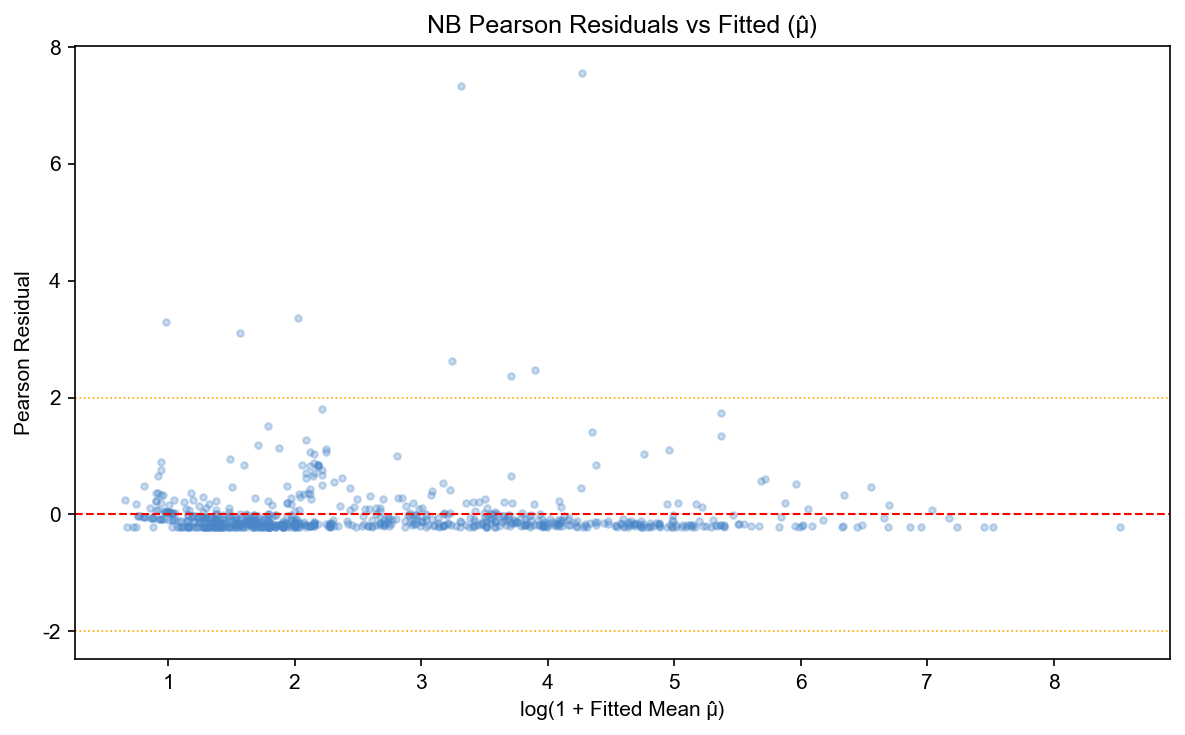
\includegraphics[width=0.78\textwidth]{../plots/nb_pearson_residuals.png}
\caption{NB Pearson 殘差對適配平均 $\hat\mu$（橘色虛線標 $\pm 2$）。殘差於整體適配範圍內以零為中心、離散度穩定；少數高適配值之觀察值落在 $\pm 2$ 之外，符合互動分布之重尾特性，並未驅動焦點係數。}
\end{figure}

\newpage

\section{OLS 視覺診斷}

\begin{figure}[H]
\centering

\includegraphics[width=0.78\textwidth]{../plots/residual_histogram.png}
\caption{OLS 殘差分布（含常態曲線疊加）}
\end{figure}

\begin{figure}[H]
\centering

\includegraphics[width=0.65\textwidth]{../plots/qq_plot.png}
\caption{OLS 殘差 Q-Q 圖}
\end{figure}

\begin{figure}[H]
\centering

\includegraphics[width=0.78\textwidth]{../plots/resid_vs_fitted.png}
\caption{OLS 殘差對適配值}
\end{figure}

\newpage

\section{相對於 v4.0.0 之比較}

\begin{table}[H]
\centering
\caption{v4.0.0（僅 OLS）與 v5.0.0（OLS + NB 穩健性）對照}
\small
\begin{tabular}{lll}
\toprule
面向 & v4.0.0 & v5.0.0 \\
\midrule
主要模型 & OLS 對數線性 & OLS 對數線性（不變） \\
穩健性模型 & --- & NB2 GLM 含 HC1 穩健 SE（新增） \\
樣本數 & $N=766$ & $N=766$（不變） \\
OLS $R^2$ & 0.5119 & 0.5119（完全複現） \\
OLS $F(8,757)$ & 76.68 & 76.68（完全複現） \\
NB 離散參數 $\hat\alpha$ & --- & 20.21（MoM 錨定） \\
LR（NB vs Poisson） & --- & $\chi^2 = 71{,}095$，$p<.0001$ \\
假說決策 & 4/5 獲支持（H1 例外） & 4/5 OLS--NB 一致；H3 於 NB 下邊際 \\
\bottomrule
\end{tabular}
\end{table}

\section{管理意涵}

\subsection{對 Booking.com 的關鍵建議}

\begin{enumerate}
    \item \textbf{擁抱簡短。}OLS 下每多一個字約 $-1.9\%$；NB 下對應 IRR $=0.97$。
    \item \textbf{靈活運用問句。}OLS 下 $\sim+60\%$；NB IRR $=2.52$（期望計數翻倍以上）。
    \item \textbf{維持正面情感基調。}OLS 下顯著（$+6.6\%$）；NB 下接近邊際（IRR $\approx 1.10$，$p=.10$），宜作為次要、軟性槓桿。
    \item \textbf{使用標籤。}OLS $\sim+189\%$；NB IRR $=2.85$，皆強且穩定。
    \item \textbf{使用 emoji。}OLS $\sim+37\%$；NB IRR $=1.47$，皆具實質效果。
    \item \textbf{務必搭配圖片。}圖片虛擬變數於兩模型中皆為最大單一效果（OLS $\sim +212\%$；NB IRR $=4.93$）。
    \item \textbf{適時 @提及合作夥伴。}@提及於兩模型中皆強（OLS $\sim+143\%$；NB IRR $=5.46$）。
\end{enumerate}

\section{研究限制與未來研究}

\begin{itemize}
    \item \textbf{觀察性橫斷面資料：}所有結論皆為相關性而非因果性。
    \item \textbf{平台特定性：}結果僅適用於 X 平台。
    \item \textbf{單一品牌：}推廣至其他旅遊品牌或產業需後續驗證。
    \item \textbf{複合互動指標：}讚、留言、分享以等權加總，未來可分項研究。
    \item \textbf{NB 離散參數識別：}重尾資料下 NB 全概似對 $\alpha$ 識別度低；本文採動差錨定方式穩健但不傳遞 $\alpha$ 不確定性至係數標準誤。
    \item \textbf{零膨脹／hurdle 模型：}本樣本零值比例 13.6\%，仍在標準 NB 適用範圍，故未估計 ZINB 或 hurdle。零值比例更高的後續樣本可加入此層穩健性。
\end{itemize}

\section{結論}

第 5.0.0 版分析確認 v4.0.0 之主要實證結論——簡短、提問、標籤、emoji、圖片以及 @提及皆為驅動 Booking.com 在 X 上互動的關鍵——並進一步在原始整數計數上加入 NB 計數模型穩健性檢驗。五項焦點假說中有四項（H1、H2、H4、H5）於 OLS 與 NB 之間一致；唯一分歧為 H3：OLS 下顯著（$p=.016$），NB 下邊際（$p=.100$），符號相同且 IRR 95\% CI 僅以薄差跨越 1。我們將此校準結果如實呈現。NB 檢驗實質強化了主要結論的推論基礎，同時對 H3 給出明確的限定條件。

\appendix
\section{技術附錄}

\subsection{軟體與套件}
\begin{itemize}
    \item Python 3、pandas、numpy、scipy、statsmodels、matplotlib。
    \item 分析腳本：\texttt{analysis/python/run\_statistics.py}（v5.0.0）。
\end{itemize}

\subsection{資料檔案}
\begin{itemize}
    \item 輸入：\texttt{data/research\_data.csv}（766 列 $\times$ 38 欄）。
    \item 輸出：\texttt{results/20260507\_155131/}（本版本）。
\end{itemize}

\section*{參考文獻}
\addcontentsline{toc}{section}{參考文獻}

\begin{enumerate}
    \item Cameron, A.C., \& Trivedi, P.K. (1990). Regression-based tests for overdispersion in the Poisson model. \textit{Journal of Econometrics}, 46(3), 347--364.
    \item Chaichi, K., John, L., \& Blackledge-Foughali, G. (2023). What makes consumers loyal to a particular online travel website? Case of booking.com.
    \item De Vries, L., Gensler, S., \& Leeflang, P.S.H. (2012). Popularity of brand posts on brand fan pages: An investigation of the effects of social media marketing. \textit{Journal of Interactive Marketing}, 26(2), 83--91.
    \item Eslami, S.P., Ghasemaghaei, M., \& Hassanein, K. (2022). Understanding consumer engagement in social media: The role of product lifecycle. \textit{Decision Support Systems}, 162, 113707.
    \item Gkikas, D.C., Tzafilkou, K., Theodoridis, P.K., Garmpis, A., \& Gkikas, M.C. (2022). How do text characteristics impact user engagement in social media posts? \textit{International Journal of Information Management Data Insights}, 2, 100067.
    \item Hudson, S., \& Thal, K. (2013). The impact of social media on the consumer decision process: Implications for tourism marketing. \textit{Journal of Travel \& Tourism Marketing}, 30(1--2), 156--160.
    \item Ko, E.E., Kim, D., \& Kim, G. (2022). Influence of emojis on user engagement in brand-related user-generated content. \textit{Computers in Human Behavior}.
    \item Kumar, N., Qiu, L., \& Kumar, S. (2022). A hashtag is worth a thousand words: An empirical investigation of social media strategies in trademarking hashtags. \textit{Information Systems Research}, 33(4).
    \item Mohammad, A.A., Elshaer, I.A., Azazz, A.M., Kooli, C., Algezawy, M., \& Fayyad, S. (2024). The influence of social commerce dynamics on sustainable hotel brand image, customer engagement, and booking intentions. \textit{Sustainability}, 16(14), 6050.
    \item Moran, G., Muzellec, L., \& Johnson, D. (2019). Message content features and social media engagement. \textit{Journal of Product and Brand Management}, 29(5), 533--545.
    \item Reddy, M.A.S., \& Prakash, C. (2024). Sentiment analysis of social media networking sites: A comparative study on user engagement and public opinion.
    \item van der Harst, J.P., \& Angelopoulos, S. (2024). Less is more: Engagement with the content of social media influencers. \textit{Journal of Business Research}, 181, 114746.
\end{enumerate}

\end{document}
